\documentclass[a4paper, 10pt]{article}
\usepackage[ascii]{inputenc}
\usepackage[T1]{fontenc}
\usepackage[romanian,english]{babel}
\usepackage{amsmath}
\usepackage{amssymb,amsfonts,textcomp}
\usepackage{color}
\usepackage{array}
\usepackage{hhline}
\usepackage{hyperref}
\hypersetup{pdftex, colorlinks=true, linkcolor=blue, citecolor=blue, filecolor=blue, urlcolor=blue, pdftitle=, pdfauthor=, pdfsubject=, pdfkeywords=}
\usepackage[pdftex]{graphicx}

%%%% Cosmin

\usepackage[a4paper, margin=2.3cm]{geometry}
\renewcommand*{\familydefault}{\sfdefault} %Sans Serif font
\renewcommand{\sfdefault}{phv} % Arial
\setlength{\parindent}{0pt} % no indentation for paragraphs
\setlength{\tabcolsep}{70pt} % table inter-column spacing

%%%%

% List styles
\newcommand\liststyleLv{%
\renewcommand\theenumi{\arabic{enumi}}
\renewcommand\theenumii{\arabic{enumii}}
\renewcommand\theenumiii{\arabic{enumiii}}
\renewcommand\theenumiv{\arabic{enumiv}}
\renewcommand\labelenumi{\theenumi.}
\renewcommand\labelenumii{\theenumii.}
\renewcommand\labelenumiii{\theenumiii.}
\renewcommand\labelenumiv{\theenumiv.}
}
\newcommand\liststyleLSi{%
\renewcommand\theenumi{\arabic{enumi}}
\renewcommand\theenumii{\arabic{enumii}}
\renewcommand\theenumiii{\arabic{enumiii}}
\renewcommand\theenumiv{\arabic{enumiv}}
\renewcommand\labelenumi{\theenumi.}
\renewcommand\labelenumii{\theenumii.}
\renewcommand\labelenumiii{\theenumiii.}
\renewcommand\labelenumiv{\theenumiv.}
}

% Footnote rule
\setlength{\skip\footins}{0.047in}
\renewcommand\footnoterule{\vspace*{-0.0071in}\setlength\leftskip{0pt}\setlength\rightskip{0pt plus 1fil}\noindent\textcolor{black}{\rule{0.25\columnwidth}{0.0071in}}\vspace*{0.0398in}}

% Pages styles
\makeatletter
\newcommand\ps@Standard{
  \renewcommand\@oddhead{}
  \renewcommand\@evenhead{}
  \renewcommand\@oddfoot{}
  \renewcommand\@evenfoot{}
  \renewcommand\thepage{\arabic{page}}
}

\makeatother
\pagestyle{plain}
\title{}
\author{}
\date{2013-04-08}

\begin{document}
{\raggedleft\bfseries
MACHETA 3
\par}

{\bfseries
Contractor: Universitatea din Bucure\c{s}ti}

{\textbf{Cod fiscal: 45055002}

\bigskip


\begin{tabular}{@{}l l}
\textbf{Avizat,}&\textbf{De acord,}\\
\textbf{Comisia de monitorizare}&\textbf{DIRECTOR PLAN SECTORIAL}\\
\\
\textbf{PRE\c{S}EDINTE:}&\\
Rolanda Predescu&\\
\\
\\
\textbf{MEMBRII:}&\textbf{MONITOR PROIECT}\\
Marioara Iordan&Daniela Dinic\u{a}\\
\\
\\
Valentina Vasile&\\
\\
\\
Speran\c{t}a P\^{a}rciog\\
\\
\\
\end{tabular}

\bigskip

\bigskip

{\centering\bfseries
RAPORT DE ACTIVITATE AL FAZEI
\par}

\bigskip

{\bfseries
Contractul nr.: 5S / 27.07.2012}

{
\textbf{Proiectul: }
\textit{`` Sistem informatic integrat pentru identificarea, arhivarea \c{s}i diseminarea bazelor de date \c{s}i a indicatorilor din
cercet\u{a}rile sociale ''}}

%TODO Numarul fazei !
%TODO Titlul fazei !
{
\textbf{Faza: }
Nr. 6 cu titlul 
\textit{`` Dezvoltare software, pachet 5: modulul de administrare, modulul de acces la date, motorul statistic ''}}

{\textbf{Termen:} 10.09.2014}

\medskip

\section{Obiectivul proiectului}

Realizarea unei arhive electronice integrate care s\u{a}
con\c{t}in\u{a} \c{s}i s\u{a} distribuie c\^at mai multe dintre 
datele sociologice acumulate \^in Rom\^ania.

\medskip

Sistemul trebuie s\u{a} ofere cercet\u{a}torilor \^in domeniul \c{s}tiin\c{t}elor sociale instrumentele necesare pentru
trecerea \^in revist\u{a}, compararea, sintetizarea, ad\u{a}ugarea datelor sociologice de interes. 
Operatorii interni ai arhivei vor c\u{a}uta, 
identifica \c{s}i acumula date sociologice disponibile \^in Rom\^ania.

\medskip

Arhiva va fi integrat\u{a} \^in Consiliul European al Arhivelor de Date Sociale (CESSDA) asigur\^andu-se un schimb
continuu bidirec\c{t}ional de informa\c{t}ie.

\section{Rezultate preconizate pentru atingerea obiectivului}

\begin{enumerate}
\item {
Sistem informatic de arhivare (stocare, catalogare plus proceduri \c{s}i capacit\u{a}\c{t}i de identificare \c{s}i
accesare) \foreignlanguage{romanian}{\c{s}}i diseminare a datelor sociale produse de pia\c{t}a cercet\u{a}rii sociale
din Rom\^ania.}
\item {
Asigurarea procedurilor de securizare a accesului la datele arhivate, ca urmare a investi\c{t}iilor \^in hardware
\foreignlanguage{romanian}{\c{s}}i software pe parcursul proiectului;}
\item {
\foreignlanguage{romanian}{Arhiva }va func\c{t}iona inclusiv ca o banc\u{a} de date sociale, dat fiind faptul c\u{a}
produc\u{a}torii de date nu au nici capacit\u{a}\c{t}ile tehnice nici \foreignlanguage{romanian}{cunoa\c{s}terea}
necesar\u{a} depozit\u{a}rii, catalog\u{a}rii \c{s}i acces\u{a}rii cercet\u{a}rilor realizate, pe termen lung;}
\item {
Facilitarea accesului comunit\u{a}\c{t}ii de cercetare din Rom\^ania la datele produse \^in ultimii 20 de ani pe
pia\c{t}a na\c{t}ional\u{a} de profil, dar \c{s}i la cele europene, ca urmare a conect\u{a}rii arhivei la CESSDA-ERIC
(arhiva fiind deja membru al CESSDA);}
\item {
Facilitarea accesului comunit\u{a}\c{t}ii de cercetare interna\c{t}ionale la datele produse \^in Rom\^ania prin
intermediul CESSDA va aduce de asemenea mari beneficii interna\c{t}ionaliz\u{a}rii cercet\u{a}rii sociale din
Rom\^ania;}
\item {
Articole de specialitate/comunic\u{a}ri \c{s}tiin\c{t}ifice menite a face cunoscute pe plan na\c{t}ional \c{s}i
interna\c{t}ional beneficiile sistemului implementat ca urmare a derul\u{a}rii sale.}
\end{enumerate}

\section{Obiectivul fazei}

%TODO Obiectivul fazei, cf. documentatiei proiectului 

\begin{itemize}
\item

\item


\end{itemize}

\section{Rezultate preconizate pentru atingerea obiectivului fazei}

%TODO Rezultate ale fazei, cf. documentatiei proiectului
Urmatoarele sisteme ale aplicatiei au fost realizate:
\begin{itemize}
\item
Modul de administrare
\item
Modul de acces la date
\item
Motor statistic
\end{itemize}

\section{Rezumatul fazei}

\medskip


\subsection{Modulul de administrare}

Modulul de administrare reprezinta ansablul de componente software
prin intermediul careia operatorii RODA intervin in functionarea sistemului.

Interfata de administrare RODA se bazeaza pe sistemul de librarii
ExtJS 4.2, sistem care permite realizarea unei aplicatii web in interiorul
programului de navigare pe internet. Astfel, interfata de administrare
RODA functioneaza foarte asemanator cu un program nativ, chiar daca
este operata cu ajutorul browserului. 

Protocolul de comunicare dintre interfata de administrare RODA si
serverul principal se bazeaza pe JSON (JavaScript Object Notation)
care este un format de reprezentare a datelor utilizat in mod special
in javascript. 

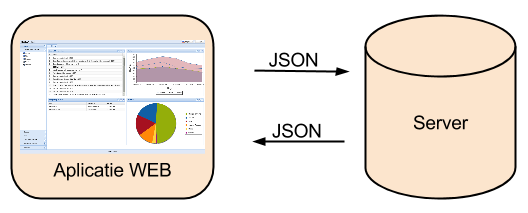
\includegraphics[width=9cm]{img/json}

\subsubsection{Componente principale ale interfetei de administrare}

\paragraph{Viewport }

Interfata de administrare ocupa toata fereastra browserului si se
redimensioneaza, impreuna cu toate componentele acesteia daca este
cazul. Acest comportament se obtine prin includerea intregii aplicatii
intr-un container special, numit viewport.

Viewportul interfetei de administrare are doua zone in care sunt incluse
componente majore: zona din partea stanga in care este inclus componentul
\textquotedblleft{}meniu\textquotedblright{} si zona centrala 

Atat meniul cat si celelalte elemente ale interfetei de administrare
sunt prezentate pe larg in anexa A. 

\paragraph{Meniu}

Meniul permite apelarea diferitelor module si submodule ale aplicatiei.
In celelalte etape ale dezvoltarii RODA au fost prezentate o serie
de module (CMS, User management, Jurnalizare, etc.). In aceasta etapa,
modulele noi sunt: Dashboard, Metadata management si modulul de management
al studiilor. Toate sunt prezentate in detaliu in anexa A. 


\paragraph{Zona centrala }

Zona centrala este un container in care se acumuleaza submodulele
deschise prin apelarea meniului. Fiecare submodul care se incarca
in zona centrala se incarca intr-un tab searat. Sistemul permite o
singura instanta a fiecarui submodul, daca acesta se apeleaza pentru
a doua oara din meniu si este deja deschis, sistemul va instrui zona
centrala sa comute afisarea pe componentul solicitat. 

\subsubsection{Modulul de management al studiilor}

Modulul de management al studiilor este cel mai complex modul din
interfata de administrare RODA si este conceput pentru a permite toate
operatiile necesare cu studiile care se gasesc in arhiva RODA. Modulul
are trei componente principale:
\begin{description}
\item [{-}] Componentul de vizualizare a studiilor existente 
\item [{-}] Editorul principal 
\item [{-}] Editorul DDI.
\end{description}
Componentul de vizualizare permite urmarirea tuturor studiilor si
a elementelor acestora. Componentul imparte ecranul in doua suprafete
distincte, una care contine lista studiilor, prezentata fie ca arbore
de cataloage, fie ca lista simpla. Respectand aceeasi paradigma vizuala
pe care o folosim in toata aplicatia RODA, la selectarea unui studiu
din lista din panoul stang, in panoul din partea dreapta si afiseaza
detaliile studiului. 

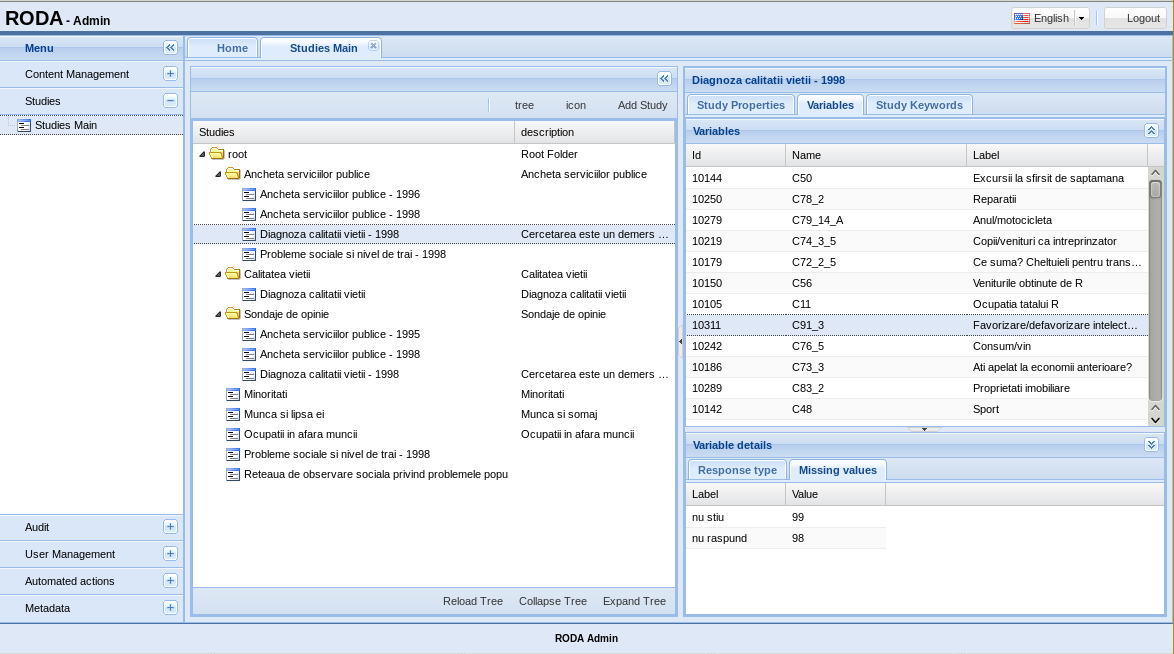
\includegraphics[width=14cm]{img/study-tree-compl}

Editorul principal permite modificarea proprietatilor studiilor existente.
Editorul principal este structurat conform standardelor de reprezentare
a datelor sociale propuse de DDI (Data Documentation Initiative).
Noile versiuni ale formatului DDI (incepand de la versiunea 3.0 in
sus) sunt concepute astfel incat sa capteze in mod distinct toate
etapele dezvoltarii unui studiu (lifecycle). Ca si interfata de vizualizare,
editorul este impartit in mai multe tab-uri, cu diferenta ca aici
toate sunt vizibile indiferent de prezenta continutului.

Editorul DDI este un set de formulare asemanatoare cu cele care alcatuiesc
componentul de editare a studiului. Editorul DDI insa este complet
separat de structura principala a bazei de date si este conceput pentru
cazurile in care un operator RODA sau un utilizator extern doreste
sa introduca un studiu in baza de date sau sa creeze un fisier in
format DDI. 

La finalizarea procesului de editare, operatorul poate semnala sistemului
ca doreste ca studiul sa fie integrat in arhiva RODA. Sistemul va
aplica o serie de validari asupra datelor si, daca verificarile determina
faptul ca datele sunt corecte, studiul este introdus in baza de date
si este sters din sistemul de stocare temporar. 

\subsection{Modul acces la date}

Modulul de accees la date este componentul care permite accesul utilizatorilor
la datele si metadatele studiilor stocate in baza de date. La fel
ca si modulul de administrare, acesta este o aplicatie WEB bazata
pe acelasi set de biblioteci, ExtJS. Introdus pentru prima data in
aplicatia RODA in a doua etapa a programarii, acesta s-a dezvoltat
odata cu aplicatia si acum permite si interfata cu motorul statistic. 

Modulul este prezentat in detaliu in Anexa A. 

\subsection{Motorul statistic}



Mai jos este prezentata o imagine a modulului de acces la date, in care se pot vedea (in partea dreapta-jos) 
si rezultatele obtinute de la motorul statistic pentru analiza unei variabile.

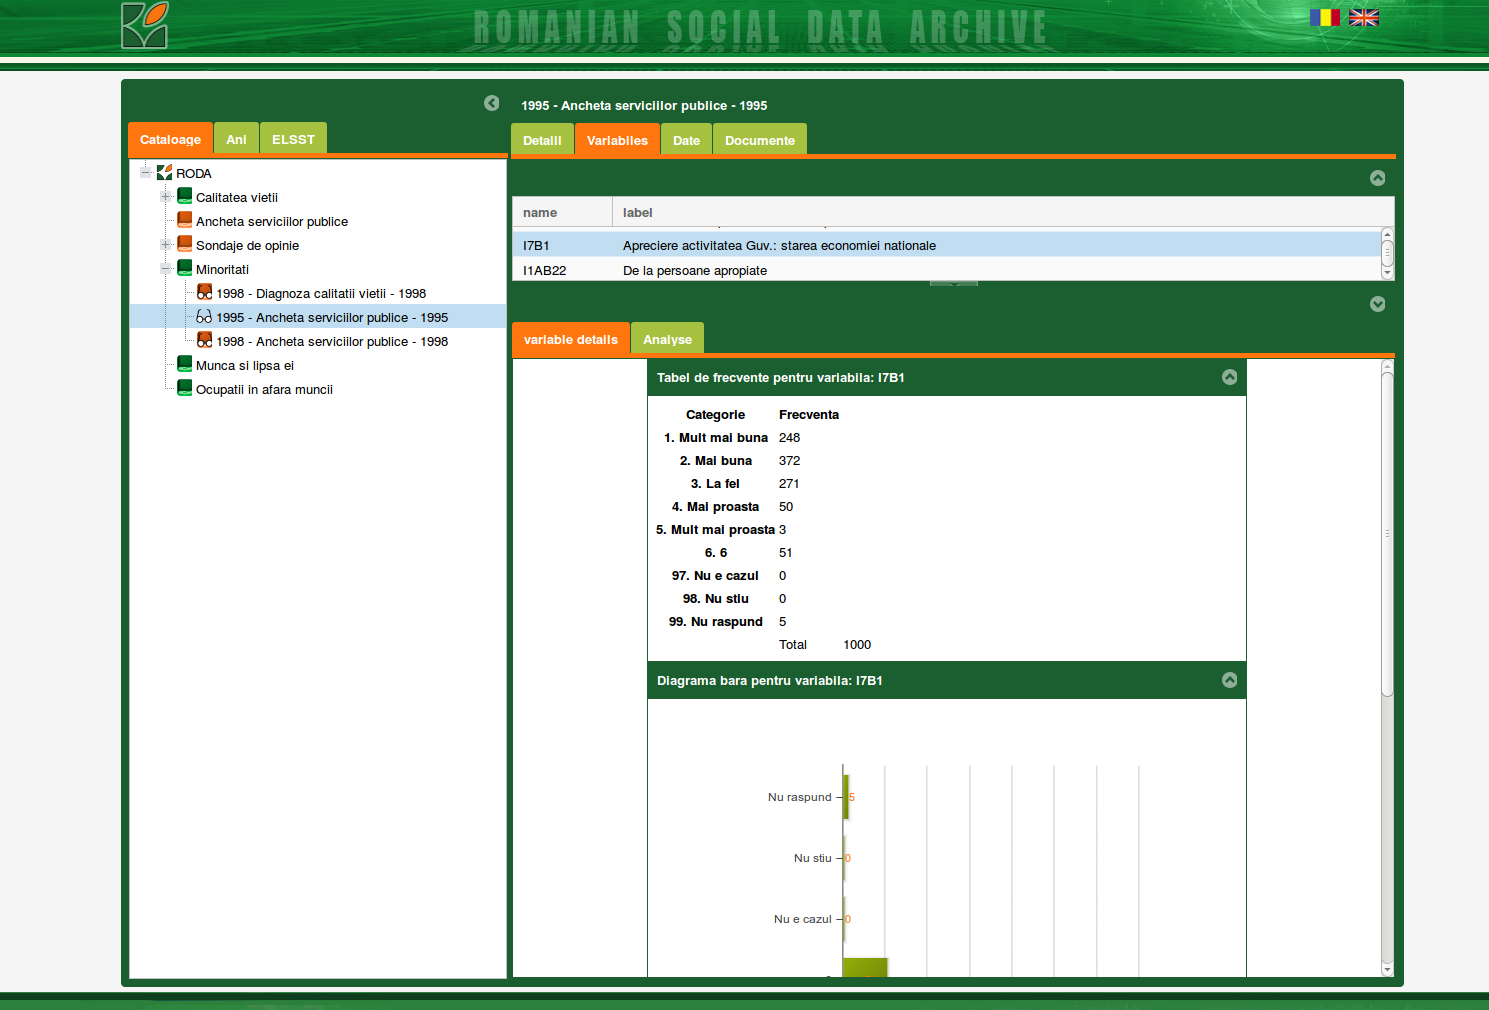
\includegraphics[width=\textwidth]{img/Screenshot-statistics}


\clearpage

\section{Rezultate, stadiul realiz\u{a}rii obiectivului, concluzii si propuneri pentru continuarea proiectului}

%TODO de completat la fiecare faza ???
Obiectivele pentru aceasta faza au fost indeplinite, fiind implementate modulul de administrare, modulul de acces la date, precum si motorul statistic.
Implementarile sunt corecte si complete, modelele de lucru cunoscute, iar interfetele permit executia tuturor operatiilor necesare pentru o buna functionare a componentelor software.


\medskip


%\clearpage

\bigskip

\bigskip

\bigskip

\bigskip

\bigskip

\bigskip

\bigskip

\bigskip

{\bfseries
RECTOR,}

prof.univ.dr. Mircea Dumitru

\bigskip

\bigskip

\bigskip

\bigskip

\bigskip

\bigskip

\bigskip

\bigskip

{\bfseries
DIRECTOR GENERAL ADMINISTRATIV,}

ec. Adrian Albu

\bigskip

\bigskip

\bigskip

\bigskip

\bigskip

\bigskip

\bigskip

\bigskip

{\bfseries
RESPONSABIL PROIECT,}

lect.univ.dr. Adrian Du\c{s}a

\end{document}
